\documentclass[]{article}
\usepackage{graphicx}
\usepackage{caption}
\usepackage{textpos}
\usepackage{float}

\usepackage[T1]{fontenc}
\usepackage[utf8x]{inputenc}
\usepackage[english]{babel}
\usepackage{hyperref}
\hypersetup{colorlinks=true}

%fancy headers
\usepackage{fancyhdr}
\pagestyle{fancy}
\fancyhf{}
\lhead{Garlic Hotel Search SRS}
\rhead{\thepage}
\usepackage{lipsum}

\title{Garlic Hotel Search SRS}
\author{James Oswald, Kyler Randall, Ethan Seligman,\\ Ed Tomlinson, Nicholas Tymeson, Paing Htet}
\date{}

\begin{document}

\maketitle
\thispagestyle{fancy}

\tableofcontents

\section{Purpose (Written by James Oswald)}
\paragraph{}
The Garlic Hotel Search aims to provide users with the ability to easily find, book, and favorite hotels. We want our application to have a clean layout, be straightforward to use without instruction, and provide fast lookup times.
\subsection{Project Background}
\paragraph{}
In the wake of the corona virus pandemic, there has been a dramatic decrease in tourism and hotel revenue worldwide. However this stands in contrast to the overwhelming statistics leading up to 2020. Statistics show that in reality hotel industry revenue was growing at an incredible average rate of 8.5\% per year, with consistent year over year growth.
\begin{figure}[H]
    \centering
    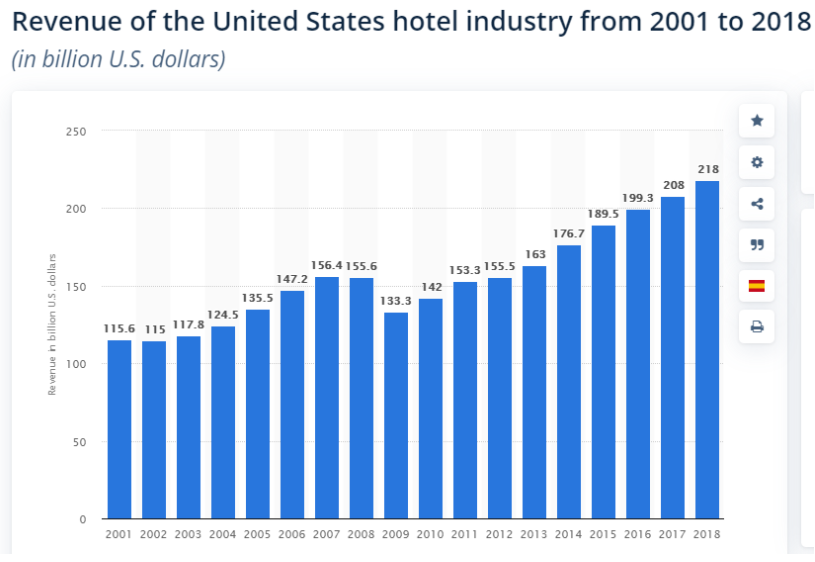
\includegraphics[scale=0.4]{hotelstats.png}
    \caption{Hotel revenue data from statistisa, source \href{https://www.statista.com/statistics/245841/total-revenue-of-the-us-hotel-industry/}{here}}
\end{figure}
\paragraph{}
We view the pandemic not as a permanent detriment, but merely as a temporary recession. We base our prediction on the figure which shows during the 2008 recession, which shows despite a drop, in 2008, the market corrected itself in just 5 years, bouncing back fully and going on to maintain consistent growth. We hope to use this correctional period as an opportunity to build a powerful tool to assist consumers in booking and finding hotels when the industry inevitably bounces back, and see this as our own opportunity to disrupt the booking industry with a powerful piece of online software. 

\subsection{Goals}
\paragraph{}
Our project has three primary service goals which help quantify how well our services meet the needs of our users:
\begin{enumerate}
    \item Easy and fast way to search hotels based off of parameters like date and location. This service goal posits that the search page must load in under 3 seconds and a search must take no longer than 5 seconds. 
    \item Ability for users to quickly book hotels. If a user knows what they want, the average time between a search and a book should be around 10 seconds. This ensures our service is straightforward and does what it's supposed to do without offering distractions.
    \item Ability for users to create accounts and favorite hotels. We will consider this feature successful if we get 1 account creation per 20 bookings. 
\end{enumerate}

\section{Stakeholders (Written by Nicholas Tymeson)}
\subsection{Our Users}
\paragraph{}
Users have a variety of needs and personal requirements when searching for hotels. The duration of their stay, like-minded customer reviews, number of people travelling, accommodating features and location, all play a crucial role in the hotel booking process. Some users may be very particular about what they’re looking for, while others may only be concerned about proximity to their destination’s attraction. Users might highly value the cleanliness of the hotel, which is a detail that would strongly influence many decisions to book or look elsewhere. Some may value accommodating features such as a fitness center, complimentary meals or service quality. Every user has a personal preference and this why hotel booking is always a process.
\subsection{User Characteristics}
\paragraph{}
Some characteristics in particular might include health/fitness oriented users, users focused on cleanliness, friendly and outgoing - might want to interact with staff, people who cook frequently, people focused on safety, and those with physical disabilities. With all of these characteristics taken into account, hotels must have a variety of accommodations such as fitness centers, handicap accessible rooms and facilities, friendly and approachable staff, mini kitchens and clean rooms.

\section{Mandated Constraints (Written by Ed Tomlinson)}
\subsection{Solution Constraints}

\subsubsection{Browser Portability}
\textbf{Description:} Garlic Hotel Search shall operate on all major internet browsers.\newline
\textbf{Rationale:} The users will use specific browsers and should not have to download a new one to operate Garlic Hotel Search.\newline
\textbf{Fit Criterion:} Garlic Hotel Search will be tested on Mozilla Firefox, Google Chrome, Safari, and Edge.

\subsubsection{Device Portability}
\textbf{Description:} Garlic Hotel Search shall operate on any screen size.\newline
\textbf{Rationale:} Users will use a specific device to view the product and should be able to view all key components.\newline
\textbf{Fit Criterion:} Garlic Hotel Search will be run on an emulator of all major screen sizes.

\subsubsection{Relevant Results}
\textbf{Description:} Garlic Hotel Search will show only relevant results from the search.\newline
\textbf{Rationale:} Users searched for specific parameters and should not see results not relevant to that search.\newline
\textbf{Fit Criterion:} All search results will match parameters given during search.

\subsubsection{Account Security}
\textbf{Description:} Garlic Hotel Search will only let clients with username and password log into a specific account.\newline
\textbf{Rationale:} User Accounts belong to a specific user and should not be accessed by others.\newline
\textbf{Fit Criterion:} The password for the account shall be unique and hashed.

\subsubsection{Personalized Results}
\textbf{Description:} Garlic Hotel Search search results will include relevant user favorited hotels.\newline
\textbf{Rationale:} A user can favorite a hotel, and that hotel should appear in future searches when relevant.\newline
\textbf{Fit Criterion:} Favorite hotels should appear in results from searches in or near their city.

\subsection{Implementation Environment}
\paragraph{}
Garlic Hotel Search shall run an internet based server. When the site is launched it will run on an internet based server so Users can access at any time. Garlic Hotel Search’s database will run on a MySQL server. The database may need to be accessed at any time. Without buying hardware to create our own database servers, a cloud based server will be the best option.

\subsection{Partner or Collaborative applications}
\paragraph{}
Garlic Hotel Search will use web data scraped from Expedia. Garlic Hotel Search does not meet the requirements necessary to use a hotel search API. Therefore we will have to scrape data from an existing site. This data will be used to complete our search requests.

\subsection{Off the shelf Software}
\paragraph{}
This is a list of OTS software used (eg bootstrap):
\begin{itemize}
    \item Garlic Hotel Search is built using \textbf{Node.js}. Node.js lets code be run concurrently and will allow multiple users to use the website simultaneously.
    \item \textbf{Express.js} is used to create Garlic Hotel Search site routing. Express.js also provides APIs and middleware used to create calls from our database and backend.
    \item  \textbf{MySQL} is used for Garlic Hotel Search’s database. MySQL is used to store our database on cloud. It can be used in the future to create powerful queries data if we create our own database of hotels and their corresponding information.
    \item \textbf{BCrypt} is used to encrypt and store user passwords in Garlic Hotel Search’s database.
    \item \textbf{Concurrently} is used to run multiple database queries simultaneously.
\end{itemize}

\subsection{Schedule}
\paragraph{}
This is a list of the remaining sprints that need to be accomplished and when:

\begin{enumerate}
    \item Sprint 2 Objectives must be completed by 10/20. Sprint 2 will ensure Garlic Hotel Search is on track. Missing objectives can be pushed to Sprint 3 but will delay the project. Too many missing objectives will affect our grade, and could affect the quality of the finished website. 
    \item Sprint 3 Objectives must be completed by 11/10. Sprint 3 is the final sprint before completion. Most objectives for Garlic Hotel Search should be completed by this deadline. Remaining time in term should be used for testing and finishing touches to the website. Any missing objectives must be completed ASAP otherwise we risk submitting an incomplete project.
    \item Garlic Hotel Search is due on 11/19. Final product must be submitted by this date. All objectives must be completed or they will not be part of the final version of Garlic Hotel Search. An incomplete project will affect the grade and could potentially be cause for the group failing.
\end{enumerate}

\section{Naming Conventions and Terms (Written by James Oswald)}

\section{Relevant Facts and Assumptions (Written by Nicholas Tymeson)}
\paragraph{Assumptions}
The following is a list of fair assumptions to make about users:
\begin{itemize}
    \item It is Fair to assume users are looking for hotels close to a particular location.
    \item It is Fair to assume users have a given price range based on the duration of their stay.
    \item It is Fair to assume users lean towards certain hotels with certain features, policies and reviews.
    \item It is Fair to assume users have a certain number of children and adults that will be staying.
\end{itemize}
  
\section{Scope (Written by Paing Htet)}
\paragraph{Use Case Diagram}
\begin{figure}[H]
    \centering
    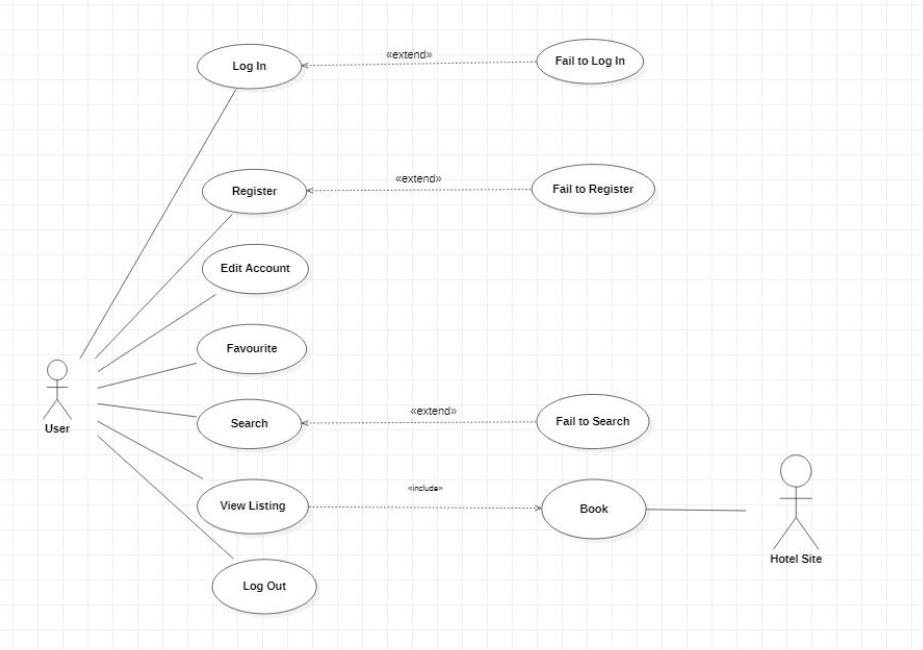
\includegraphics[scale=0.4]{usecase.png}
    \caption{Our Updated Use Case Diagram}
\end{figure}

\end{document}
